\chapter{Framework}
\section{Introduction}
In [Insert Book] it was shown that some integer linear programs (ILPs) could be solved by constructing some directed and weighted graph and finding the shortest path between 2 special vertecies. If $A\vec x = \vec b$, $A\in \N^{m \times n}, \vec x \in \N^n, \vec b \in \N^m$ is the given ILP, only those ones were discussed, where in $A$ all columns would sum up to the same number. The resulting algorithm has polynomial runtime when we fix the dimension $m$. We will revisit this approach and extend it to $A\in\Z^{m \times n}$, where the column sums in $A$ are allowed to be different but must be strictly positive. This will be achieved by first translating the given ILP into a one, that can be handled by the algorithm proposed by [Name einfügen] and then performing this algorithm. This trabnslation will yield a degree of freedom, which will non-trivially influence the performance of the final algorithm. The main part of this thesis will discuss possibilities to use the degree of freedom. 

\section{The semiring}
\begin{definition}
    A \textit{semiring} $(S, \oplus, \odot, 0, 1)$ consist of the \textit{carrier set} $S$, two binary operations $\oplus$,$\odot$ and two special elements $1, 0 \in S$, such that for all $a, b, c \in S$ hold the following properties:
    \begin{align*}
        a \oplus b &= b \oplus a &&\textrm{Commutivity of $\oplus$}\\
        (a \oplus b) \oplus c &= a \oplus (b \oplus c) &&\textrm{Associativity of $\oplus$}\\
        (a \odot b) \odot c &= a \odot (b \odot c) &&\textrm{Associativity of $\odot$}\\
        a \oplus 0 &= a &&\textrm{Neutral Element of $\oplus$}\\
        a \odot 1 = 1 &\odot a = a &&\textrm{Neutral Element of $\odot$}\\
        a \odot 0 = 0 &\odot a = 0 &&\textrm{0 absorbs for $\odot$}\\
        a \odot (b \oplus c) &= (a \odot b) \oplus (a \odot c) &&\textrm{Distributivity}\\
        (a \oplus b) \odot c &= (a \odot c) \oplus (b \odot c)
    \end{align*}
\end{definition}

In contrast to the ordenary ring, the semiring lacks the additive inverses. Thus every ring and thereby every field is a semiring. More important semirings include $(\R \cup \{-\infty\}, \max, +, -\infty, 0)$ or the \textit{tropical semiring} $(\R \cup \{\infty\}, \min, +, \infty, 0)$.

\begin{definition}
    Given a semiring $(S, \oplus, \odot, 0, 1)$ we can construct the semiring of square matrix operations \textit{induced by $S$}, resulting in the semiring $(S^{n \times n}, \boxplus, \boxdot, \zeromat, \imat)$, with:
\begin{align*}
    (A \boxplus B)_{ij} &= A_{ij} \oplus B_{ij}\\
    (A \boxdot B)_{ij} &= (A_{i1} \odot B_{1j}) \oplus (A_{i2} \odot B_{2j}) \oplus \dots \oplus (A_{in} \odot A_{nj})\\
    \zeromat_{ij} &= 0\\
    \imat_{ij} &= \begin{cases}
        1 &\textrm{if}\quad i = j\\
        0 &\textrm{else}
    \end{cases}
\end{align*}
\end{definition}

Remember that the use of 1 and 0 revers to the special elements in the semiring. For example the identity matrix induced by the tropical semiring look like this:
$$
\left(
\begin{matrix}
    0 & \infty & \infty & \dots & \infty\\
    \infty & 0 & \infty & \dots & \infty\\
    \infty & \infty & 0 & \dots & \infty\\
    \vdots & \vdots & \vdots & \ddots & \vdots\\
    \infty & \infty & \infty & \dots & 0
\end{matrix}
\right)
$$
\begin{definition}
    An operation $*\colon S \times S \to S$ is called $idempotent$ iff 
    $$\forall a \in S: a * a = a$$
\end{definition}
\begin{example}
    $\min$ and $\max$ are idempotent, because $\forall n \in \N\colon \max\{a, a\} = \min\{a, a\} = a$. This means that in the tropical semiring the $\oplus$-operation is idempotent.
\end{example}

\section{Graphs}
\begin{definition}
    A \textit{graph} $G = (V, E)$ consist of a set of \textit{vertices} $V$ and a set of \textit{edges} $E$. In a \textit{directed graph} $E \subseteq V \times V$, in an \textit{undirected graph} $E \subseteq \binom{V}{2}$. 
\end{definition}
\begin{figure}[ht]
    \centering
    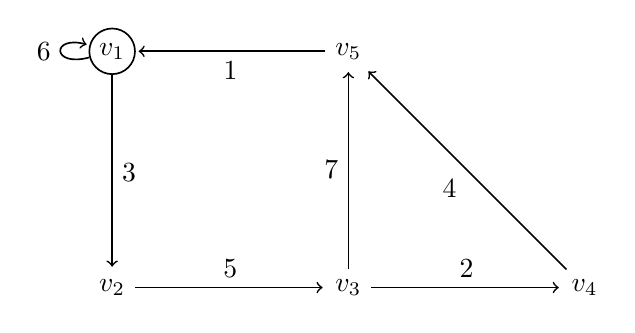
\begin{tikzpicture}[->,shorten >=1pt,auto,node distance=3cm,semithick]

    
      \node[circle, draw, fill=white, inner sep=2pt] (v1) {$v_1$};
      \node (v2) [below of=v1] {$v_2$};
      \node (v3) [right of=v2] {$v_3$};
      \node (v5) [right of=v1] {$v_5$};
      \node (v4) [right of=v5, below of=v5] {$v_4$};
    
      \path (v1) edge node {3} (v2)
            (v2) edge node {5} (v3)
            (v3) edge node {2} (v4)
            (v4) edge node {4} (v5)
            (v5) edge node {1} (v1)
            (v1) edge [loop left] node {6} (v1)
            (v3) edge node {7} (v5);
    \end{tikzpicture}
    \caption{Weighted Directed Graph with 5 Nodes}
\end{figure}

\begin{align*}
    A = \begin{bmatrix}
    \infty & 3 & \infty & \infty & \infty \\
    \infty & \infty & 5 & \infty & \infty \\
    \infty & \infty & \infty & 2 & 7 \\
    \infty & \infty & \infty & \infty & 4 \\
    1 & \infty & \infty & \infty & \infty \\
    \end{bmatrix}
\end{align*}
\section{Einsums}
\subsection{Definition}
\subsection{Common examples}
\subsection{Properties}